\documentclass[a4paper]{article}

\usepackage{color}
\usepackage{url}
\usepackage[T2A]{fontenc} % enable Cyrillic fonts
\usepackage[utf8]{inputenc} % make weird characters work
\usepackage{graphicx}
\usepackage{indentfirst}
\usepackage[english,serbian]{babel}


\usepackage[unicode]{hyperref}
\hypersetup{colorlinks,citecolor=green,filecolor=green,linkcolor=blue,urlcolor=blue}

\usepackage{listings}

\newtheorem{primer}{Primer}[section]

\definecolor{mygreen}{rgb}{0,0.6,0}
\definecolor{mygray}{rgb}{0.5,0.5,0.5}
\definecolor{mymauve}{rgb}{0.58,0,0.82}

\lstset{ 
  backgroundcolor=\color{white},   % choose the background color; you must add \usepackage{color} or \usepackage{xcolor}; should come as last argument
  basicstyle=\scriptsize\ttfamily,        % the size of the fonts that are used for the code
  breakatwhitespace=false,         % sets if automatic breaks should only happen at whitespace
  breaklines=true,                 % sets automatic line breaking
  captionpos=b,                    % sets the caption-position to bottom
  commentstyle=\color{mygreen},    % comment style
  deletekeywords={...},            % if you want to delete keywords from the given language
  escapeinside={\%*}{*)},          % if you want to add LaTeX within your code
  extendedchars=true,              % lets you use non-ASCII characters; for 8-bits encodings only, does not work with UTF-8
  firstnumber=1000,                % start line enumeration with line 1000
  frame=single,	                   % adds a frame around the code
  keepspaces=true,                 % keeps spaces in text, useful for keeping indentation of code (possibly needs columns=flexible)
  keywordstyle=\color{blue},       % keyword style
  language=Python,                 % the language of the code
  morekeywords={*,...},            % if you want to add more keywords to the set
  numbers=left,                    % where to put the line-numbers; possible values are (none, left, right)
  numbersep=5pt,                   % how far the line-numbers are from the code
  numberstyle=\tiny\color{mygray}, % the style that is used for the line-numbers
  rulecolor=\color{black},         % if not set, the frame-color may be changed on line-breaks within not-black text (e.g. comments (green here))
  showspaces=false,                % show spaces everywhere adding particular underscores; it overrides 'showstringspaces'
  showstringspaces=false,          % underline spaces within strings only
  showtabs=false,                  % show tabs within strings adding particular underscores
  stepnumber=2,                    % the step between two line-numbers. If it's 1, each line will be numbered
  stringstyle=\color{mymauve},     % string literal style
  tabsize=2,	                   % sets default tabsize to 2 spaces
  title=\lstname                   % show the filename of files included with \lstinputlisting; also try caption instead of title
}

\begin{document}

\title{Vizuelizacja simboličkog izvršavanja\\ \small{Seminarski rad u okviru kursa\\Verifikacija softvera\\ Matematički fakultet}}

\author{Aleksandra Kovačević, \\Nikola Stojević, \\Kristina Stanojević\\ \\aleksandrakovacevic099@gmail.com, \\nikolastojevic@gmail.com, \\stanojevic.kristina@gmail.com}

%\date{20.~april 2019.}

\maketitle

\abstract{
U ovom tekstu je ukratko objašnjeno korišćenje programa \textbf{sym\_tree.py} koji pomoću alata \textit{Klee} \cite{Klee} vrši vizuelizaciju simboličkog izvršavanja nekog programa napisanog u programskom jeziku \textit{C}. Klee služi za simboličko izvršavanje programa i za automatsko generisanje test primera. Koristeći fajlove koje izgeneriše iscrtavaćemo drvo simboličkog izvršavanja. Takodje postoji opcija za iscrtavanje stabla do zadate dubine, u slučaju da je prosledjeni program koji analiziramo previše kompleksan, ili nas zanima samo odredjeni deo instrukcija. 
}


\tableofcontents

\newpage

\section{Skup fajlova i način pokretanja programa}

Pre korišćenja programa potrebno je instalirati odgovarajuće alate (\textit{clang} \cite{clang}, Klee, ...). Spisak tih instalacija nećemo redom navoditi u ovom radu. Osnova jesu oni alati koji se koriste u okviru kursa \textit{Verifikacija softvera} na Matematičkom fakultetu u Beogradu.

\subsection{Pokretanje}

Pored osnovnih instalacija, u fajlu \textbf{requirements.txt} navedeno je šta je još neophodno imati kako bi dati program radio. To se može instalirati pokretanjem sledeće linije:

\textbf{pip install -r requirements.txt} \\

Pokretanje samog programa je olakšano skriptom \textbf{makeTree.sh}. Najpre je potrebno da se omogući izvršavanje te skripte kao i samog programa korišćenjem komande:

\textbf{chmod +x \&\& chmod +x makeTree.sh} \\

Nakon tih koraka sledećom komandom pokrećemo naš program: 

\textbf{./makeTree.sh \{absolute\_path\_to\_c\_file\}\\ \{absolute\_path\_to\_where\_you\_want\_your\_sym\_tree\_image\} } 

Primer pokretanja:\\ \textit{./makeTree.sh /Downloads/07\_materijali/pointer\_error\_sym.c /Downloads/drvo }, nakon čega dobijamo fajlove \textit{drvo.pdf} i \textit{drvo.gv} kao rešenje. Način korišćenja se može videti i jednostavnim pokretanjem \textit{./makeTree.sh -h}.


\subsection{Ukratko o koracima}

Izvršavanje alata Klee za sobom ostavlja fajlove koje smo koristili za iscrtavanje. U odgovarajućim fajlovima sa ekstenzijom \textbf{.pc} nalaze se instrukcije napisane u obliku koji nama nije odgovarajući za čitljivo ispisivanje instrukcija u čvorovima stabla. Zato je potrebno prilagoditi ispis korišćenjem parsera \textbf{parser.py} koji se nalazi u folderu \textbf{Parser}. Vrši se analiza, parsiranje i odgovarajuće iscrtavanje stabla, sa detaljima o putanjama u okviru čvorova, koje je dato u PDF fajlu kreiranom nakon izvršavanja. Detaljno objašnjenje svake linije koda neće biti dato u tekstu.

\subsection{Drugi način pokretanja}
Ukoliko dodje do nekih grešaka u toku pokretanja skripte \textit{makeTree.sh}, moguće je samostalno pokretati jednu po jednu liniju u sledećem poretku kako bi se došlo do istog krajnjeg cilja:\\

\begin{itemize}
    \item {Generisanje llvm koda: \textbf{myclang -I \{path\_to\_klee\_include\} -emit-llvm -c -g \{name\_of\_the\_file\}.c}, nakon čega dobijamo \{name\_of\_the\_file\}.bc fajl}
    
    \item {Prepuštanje dobijenog fajla Klee alatu: \textbf{myklee --write-sym-paths --write-pcs \{name\_of\_the\_file\}.bc}, nakon čega dobijamo odgovarajuće foldere sa test primerima i putanjama}
    
    \item {Pokretanje našeg python koda za kreiranje stabla: \textbf{python3 sym\_tree.py -d 10}}
\end{itemize}


\section{Primer rezultata}
Na slici \ref{fig:primer} prikazan je jedan rezultat dobijen analizom nekog C programa. U čvorovima su ispisani uslovi koji se ispituju, grane su obeležene kao \textit{t} ili \textit{f} ako pretstavljaju da li je u toj putanji uslov iz čvora ispunjen ili ne. U listovima oznaka \textit{end} predstavlja kraj jedne od putanja.

\begin{figure}[h!]
\begin{center}
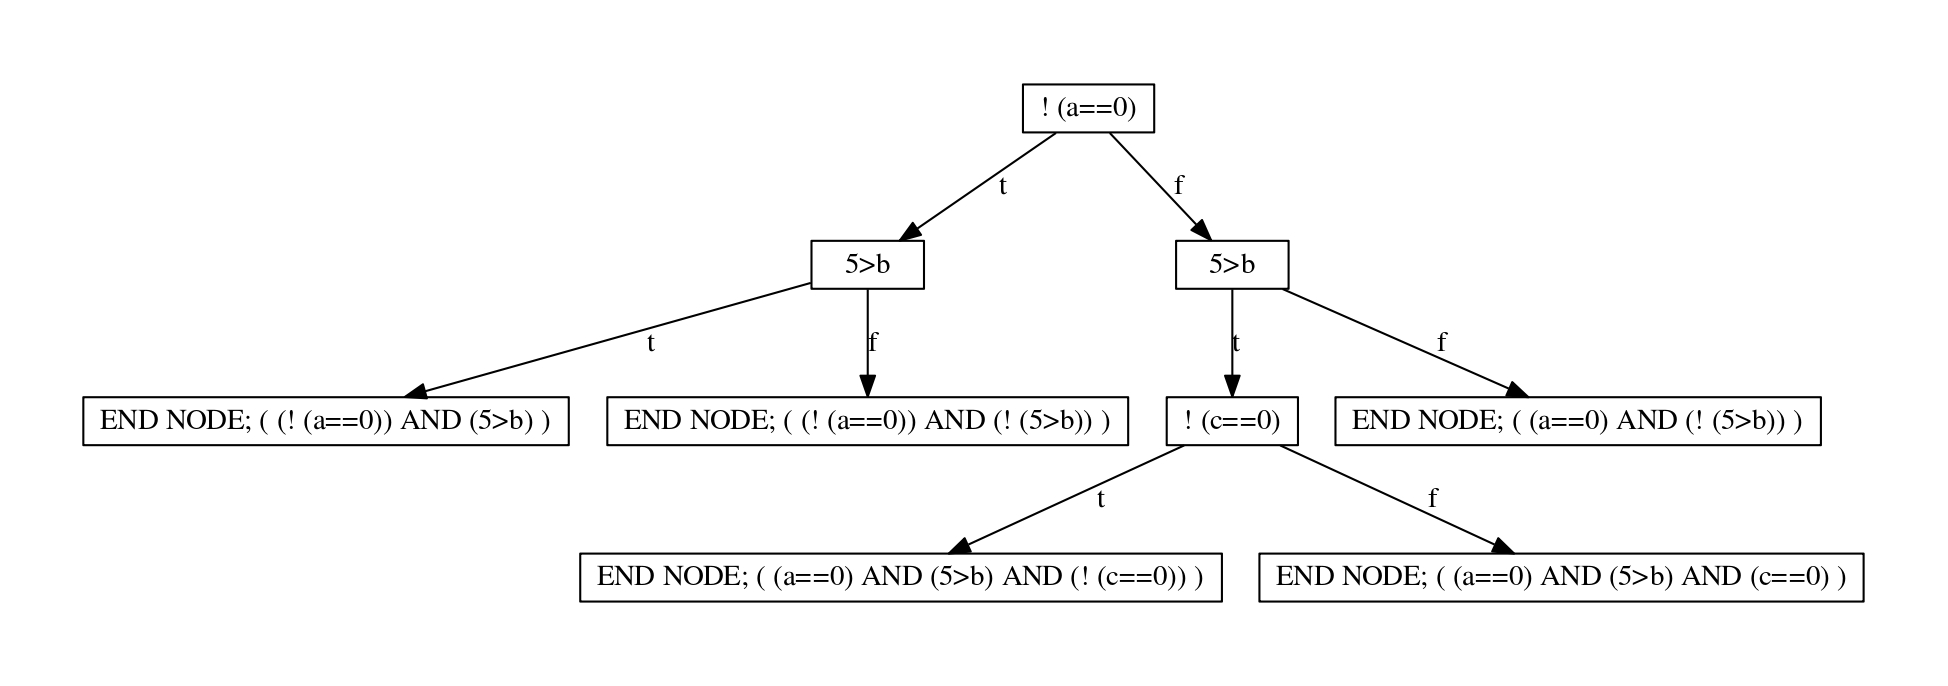
\includegraphics[scale=0.6]{primer.jpg}
\end{center}
\caption{Primer jednog stabla simboličkog izvršavanja}
\label{fig:primer}
\end{figure}

\addcontentsline{toc}{section}{Literatura}
\appendix
\bibliography{seminarski} 
\bibliographystyle{plain}


\end{document}